\subsection{Controller Performance}
The performance of the controller can be seen in \autoref{fig:xbdot_lqr} and \ref{fig:yaw_lqr}. 
\begin{figure}[H]
    \captionbox 
    {   
        Step response of the model with linear quadratic regulator in $\dot{x}_\mathrm{b}$.
        \label{fig:xbdot_lqr}
    }                                                                 
    {                                                                  
        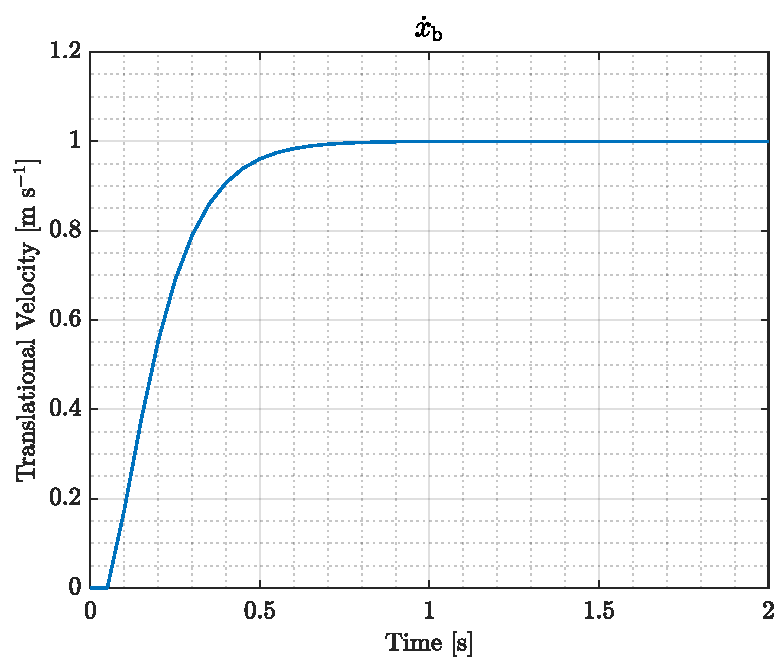
\includegraphics[width=.45\textwidth]{figures/xbdot_lqr}         
    }                                                                    
    \hspace{5pt}                                                          
    \captionbox  
    {      
        Step response of the model with the linear quadratic regulator in $\psi$ at 10 s.
        \label{fig:yaw_lqr}
    }                                                                          
    {
        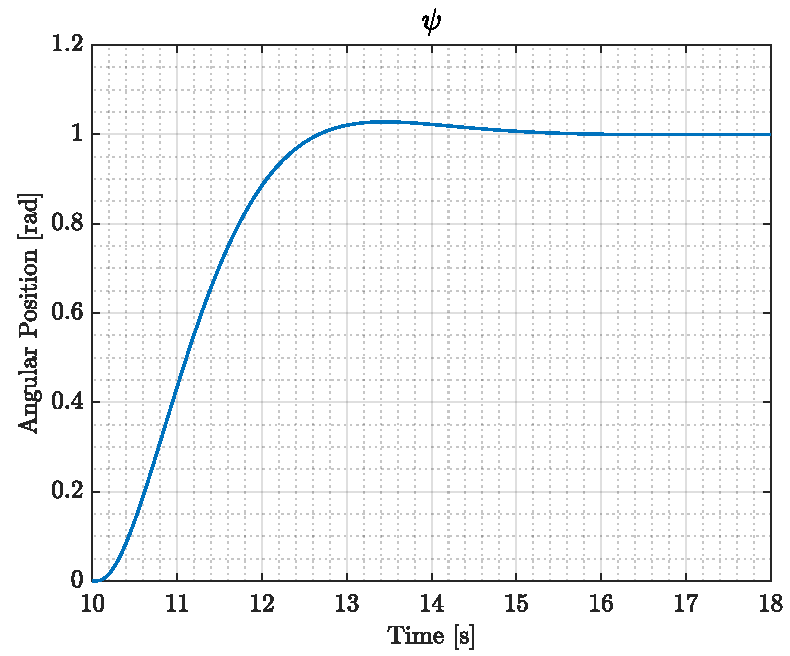
\includegraphics[width=.45\textwidth]{figures/yaw_lqr}
    }
\end{figure}
%
In the simulation, a step reference is set to $\dot{x}_\mathrm{b}$ and then a reference is set to $\psi$ at 10 s. This is done to analyze the behavior closed ot real conditions, when the boat is turning while having constant speed.

It can be seen in \autoref{fig:xbdot_lqr} that the settling time, with an error band of 5 \%, for $\dot{x}_\mathrm{b}$ is around \num{0.5} s. There is not overshoot until the response is disturbed when the reference for $\psi$ is set, but it recovers in less than \num{0.2} s.

The response in $\psi$, \autoref{fig:yaw_lqr}, has a settling time of \num{2.2} s and an overshoot of less than 5 \%.

\fxnote{Check seconds and settling times with final graphs in LQR simulations}